\documentclass[a4paper,11pt]{report}

% General tools
\usepackage{etoolbox}

\usepackage[utf8]{inputenc}

% Fonts
\usepackage[T1]{fontenc}

% LaTeX modern fonts
\usepackage{lmodern}

% Sans serif
%\usepackage{tgheros}

% Serif
%\usepackage[bitstream-charter]{mathdesign}

% Monospace
%\usepackage{sourcecodepro}

% Language
\usepackage[english]{babel}
\usepackage{blindtext}
\usepackage{url}

% Page style
\usepackage{fullpage} % page margins to 1.5cm
\usepackage{fancyhdr} % headers and footers

% Colors & graphics
\usepackage[table]{xcolor}    % colors
\usepackage[pdftex]{graphicx} % graphics importing

% Misc
\usepackage{titlesec} % section titles formatting
\usepackage{minted}   % code highlighting
\usepackage{lscape}   % landscape
\usepackage{tikz}     % charts in LaTeX
\usepackage{amsmath}  % better math
\usepackage{float}    % floats
\usepackage[small,justification=centering]{caption}
\usepackage{microtype} % typographic improvements

% Paragraphs
\usepackage{parskip}
\usepackage[defaultlines=3,all]{nowidow}

% Chapter titles
% Remove space before title
\titlespacing{\chapter}{0pt}{*-4}{*3}
% Remove "Chapter N" and use a sans-serif font
\titleformat{\chapter}[hang]{\bf\huge}{\thechapter}{1pc}{}
% Change chapter page style
\patchcmd{\chapter}{plain}{fancy}{}{}

% Tables
\usepackage{multirow}

% Cross-references
\usepackage{hyperref}


% Metadata for this report
% ------------------------
\newcommand{\School}{University of Applied Sciences Western Switzerland}
\newcommand{\Faculty}{MSE - Software Engineering}
\newcommand{\Place}{Lausanne}

% Course

\newcommand{\Title}{<Title>}

% Supervisors (professors)
\newcommand{\Supervisors}{Prof. Carlos Peña}

% Students
\newcommand{\Authors}{Déruaz Vincent}

%TOOLS
\newcommand{\todo}[1]{\textcolor{red}{TODO: #1}\PackageWarning{TODO:}{#1!}}

\newcommand{\Course}{Projet d'approfondissement \\ Inphinity}


% Header and footer
% -----------------
\pagestyle{fancy}
\lhead[]{\Course}
\chead[]{}
\rhead[]{\Place, \today}

\setlength{\headheight}{14pt}
\setlength{\headsep}{14pt}

\newcommand{\HRule}{\rule{\linewidth}{0.5mm}}

% Code styles for highlighting
% ----------------------------

% How to use (replace 'java' with language name):
% - code blocks:
%     \begin{javacode}
%     CODE
%     \end{javacode}
% - files:
%     full: \javafile{PATH}
%     extract: \javafile[startline=x, endline=y]{PATH}
% TODO: inline?

% Java
\newminted{java}{frame=single, framesep=6pt, breaklines=true, fontsize=\scriptsize}
\newmintedfile{java}{frame=single, framesep=6pt, breaklines=true, fontsize=\scriptsize}

% Scala
\newminted{scala}{frame=single, framesep=6pt, breaklines=true, fontsize=\scriptsize}
\newmintedfile{scala}{frame=single, framesep=6pt, breaklines=true, fontsize=\scriptsize}

% Python
\newminted{python}{frame=single, framesep=6pt, breaklines=true, fontsize=\scriptsize}
\newmintedfile{python}{frame=single, framesep=6pt, breaklines=true, fontsize=\scriptsize}

% Plain text
\newminted{text}{frame=single, framesep=6pt, breaklines=true, breakanywhere, fontsize=\scriptsize}
\newmintedfile{text}{frame=single, framesep=6pt, breaklines=true, breakanywhere, fontsize=\scriptsize}

% Document
% --------
\begin{document}

\begin{titlepage}
    \begin{center}

        % only works if a paragraph has started.
        
\includegraphics[width=0.8\textwidth]{img/mse_logo}~\\[1.5cm]
        \textsc{\Large \School}\\[0.25cm]
        \textsc{\Large \Faculty}\\[1.5cm]

        % Title
        \HRule \\[0.4cm]
        { \huge \bfseries \Course \\[0.4cm] }
        \HRule \\[1.5cm]

        % Author and supervisor
        \begin{minipage}[t]{0.4\textwidth}
            \begin{flushleft} \Large
                \emph{Authors:}\\ \Authors
            \end{flushleft}
        \end{minipage}
        \begin{minipage}[t]{0.4\textwidth}
            \begin{flushright} \Large
                \emph{Supervisors:}\\\Supervisors
            \end{flushright}
        \end{minipage}~\\[1.5cm]

        \begin{center}
            
\includegraphics[scale=0.7]{img/logo_hes-so}
        \end{center}

        \vfill

        % Bottom of the page
        {\large \Place, \today}

    \end{center}
\end{titlepage}

\tableofcontents


\chapter{Introduction}
\section{foreword}
This project falls within the context of a thesis proposed by Prof. Carlos Peña, YokAi
Que, MDPhD and Grégory Resch, PhD entitled \textit{In silico prediction of phagebacteria
infection networks as a tool to implement personalized phage therapy} \cite{ref1}.

The official statment of the project is:\\
By using automated learning methods, explore alternate metodologies for bacteria and phages interaction modelisation on genomic informations or proteins.


\section{phages Vs bacteria}
In our modern world a challenging issues has apear concerning conventional antibiotics. In deed, some batceria have developpe resistance to antibiotics. To overcome this people are looking at phage therapy. 

Phage therapy is the utilisation of phages, bacteriophage viruses, to threat infectious diseases of bacterial origin. This therapy is known to have only very few and only benign side effets. This last point make phagotherapy, not only useful to avoid antibiotic in case of resistance, but also to avoid their "toxicity".

Briefly, phage therapy was the only threatment solution in the before the 1930's. The apearence of the penicillin in the early 1940's and other modern drugs, releagate phage therapy to the past. But, in the slavic countries, phage therapy continued to be used as a current treatment.

Luckly for us, we don't have to start from nothing in phage therapy. However, we have the necessity to find a way, a methode to validate the phage selection. \cite{ref2}




\chapter{State of the art}

\section{Biology}
\todo genome


\section{Bio-informatic}
\todo sequence alignment

\todo explain phamily

\todo explain genebank


\chapter{Methods}
In this section we will disscuss about what we've used during this project. The Docker technology is used to build the differents work enviornment. Phamerator and PhamDB are used to compute genomes into phamily. Everythings is stored into some Sql databases.

\section{Docker}
Docker allows to package applications with a fonctionnal system and every dependencies needed to run it, into a standardized container. \cite{ref3}

\subsection{Functionment}
In a specific file called 'Dockerfile' you describe a system. You can build and run this system everywhere docker engine is installed. It will create a container, containing your application.

Container are an isolated system from host or other containers. You can use every Linux distribution to run your container.

Docker build images using layers, it allows docker to share those layer between containers, reducing disk usage at best.

\begin{figure}
	\begin{center}
		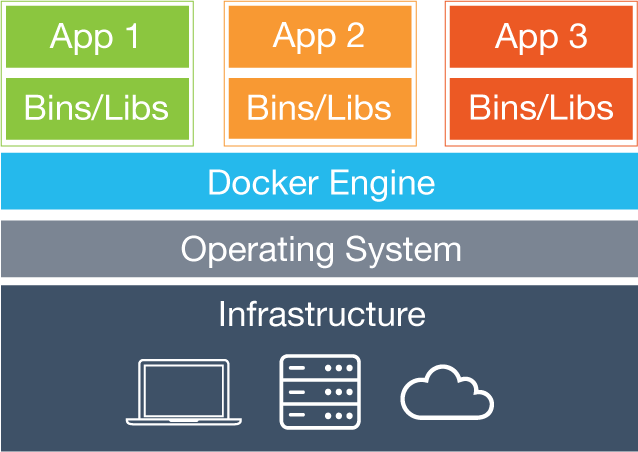
\includegraphics[scale=0.35]{img/what-is-vm-diagram}
		\caption{Docker harchitecture}
	\end{center}
\end{figure}

\subsection{Docker-machine installation}
you have to install docker on your system, it can be used on Linux, Windows or MacOs. \url{https://docs.docker.com/linux/}

\subsubsection{Windows}
If you want to use docker on Windows you need to do as folowing to ensure to have a docker-machine with more than 20Go.

\begin{javacode}
$ docker-machine rm default
$ docker-machine create -d virtualbox --virtualbox-memory=4096 --virtualbox-cpu-count=2 --virtualbox-disk-size=50000 default
\end{javacode}

It will crate a docker-machine with 50Go of disk space.

\subsection{Docker commands}
Here are the basic commands you will need to manage docker. Attention, you will need to be in the same directory as the Dockerfile.

This command allow to build an image describe in the Dockerfile.
\begin{javacode}
$ docker build -t "<image Name>" .
\end{javacode}

This command is used to run a container using a pre-build image, with a binding port.
\begin{javacode}
$ docker run -it -d -p <host port>:<container port> <image name>
\end{javacode}

If you need to acces the container bash console, juste use this commande
\begin{javacode}
$ docker exec -i -t <container ID> /bin/bash
\end{javacode}

You can list all the running containers and use a <container id> to stop it.
\begin{javacode}
$ docker ps
$ docker stop <container ID>
\end{javacode}

This last command give you the ip of your docker-machine.
\begin{javacode}
$ docker-machine ip
\end{javacode}

\subsection{Inphinity, build \& run}
For the main code of this project we use python through Jupyter. To do so you can find a docker image that run Jupyter, python3 and some machin learning libraries. go to "dockers/jupyter\_align\_mysql" directory.

To build and run the environment type the following commands:
\begin{javacode}
$ docker build -t "pa/inphinity" .
$ docker run -v <path to project dir>/jupyter_align_mysql/src:/home/pa/work/ -i -t -d -p 8888:8888 pa/inphinity
\end{javacode}

Replace <path to project dir> by the entire path to the directory. If you want to, you can change the host port. Just change "\textit{-p 8888:8888}" to "\textit{-p <any port>:8888}".

You can now acces the jupyter interface and the project files using any browser you want using \url{http://<docker-machine ip>:8888}

At this point you should see the interface figue 3.2

\begin{figure}[H] 
	\begin{center}
		
\includegraphics[scale=0.45]{img/login_jupyter}
		\caption{Jupyter login page}
	\end{center}
\end{figure}

\textbf{Rq:} The password is "Inphinity-more"

When you're logged in you can access the "inphinity" directory. It contains most of this project results. We will disscuss them later in this document.

\begin{figure}[H] 
	\begin{center}
		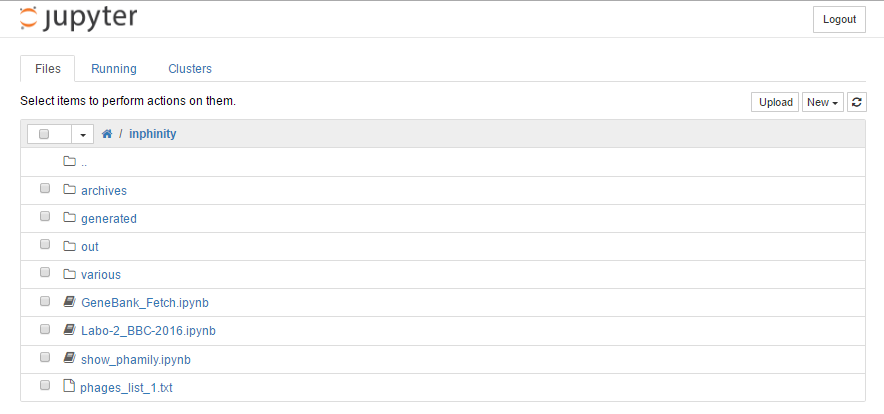
\includegraphics[scale=0.45]{img/inphinity_jupyter}
		\caption{Inphinity jupyter directory}
	\end{center}
\end{figure}

\section{Phamerator}
Phameraotr is \textit{a bioinformatic tool for comparative bacteriophage genomics} \cite{ref4}. Phamerator will allow us to compute and store phamily, in a database. 

\subsection{Installation}
\todo install on GUI machine

\subsection{How it's works}
\todo screens + explain

\section{PhamDB}
To facilited the construction of databases containing our phamily we will use PhamDb. In deed, with phamDb we can populate a database with new phage. At every addition of phage, it will recompute phamily accordingly to the new phage added. 

We no longer need to access to Phamerator by GUI. In the future it will let us build a fully automated pipline of actions.

\subsection{Installation \& Run}
To build and run the environment type the following commands:
\begin{javacode}
$ docker build -t "pa/phamdb" .
$ docker run -v <path to project dir>/jupyter_align_mysql/src:/home/pa/work/ -i -t -d -p 81:80 pa/phamdb
\end{javacode}

Replace <path to project dir> by the entire path to the directory. If you want to, you can change the host port. Just change "\textit{-p 81:80}" to "\textit{-p <any port>:80}".

You can now acces the jupyter interface and the project files using any browser you want using \url{http://<docker-machine ip>:80}

At this point you should see the interface figue 3.4, but with no database for the moment.

\begin{figure}[H] 
	\begin{center}
		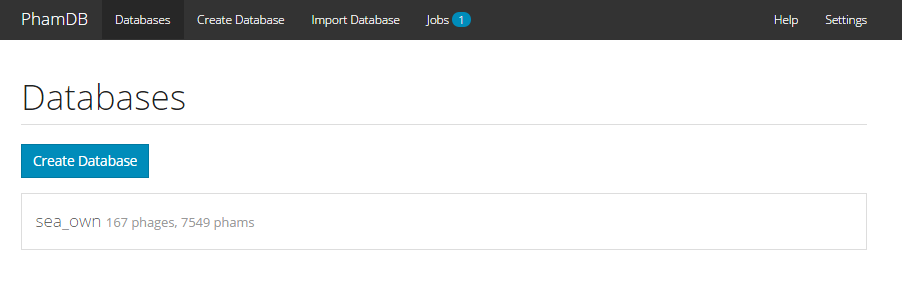
\includegraphics[scale=0.45]{img/phamdb}
		\caption{Phamdb interface}
	\end{center}
\end{figure}

\subsection{Utilisation}
As you see from figure 3.4 you can access the list of all existing database and consult them.

\begin{figure}[H] 
	\begin{center}
		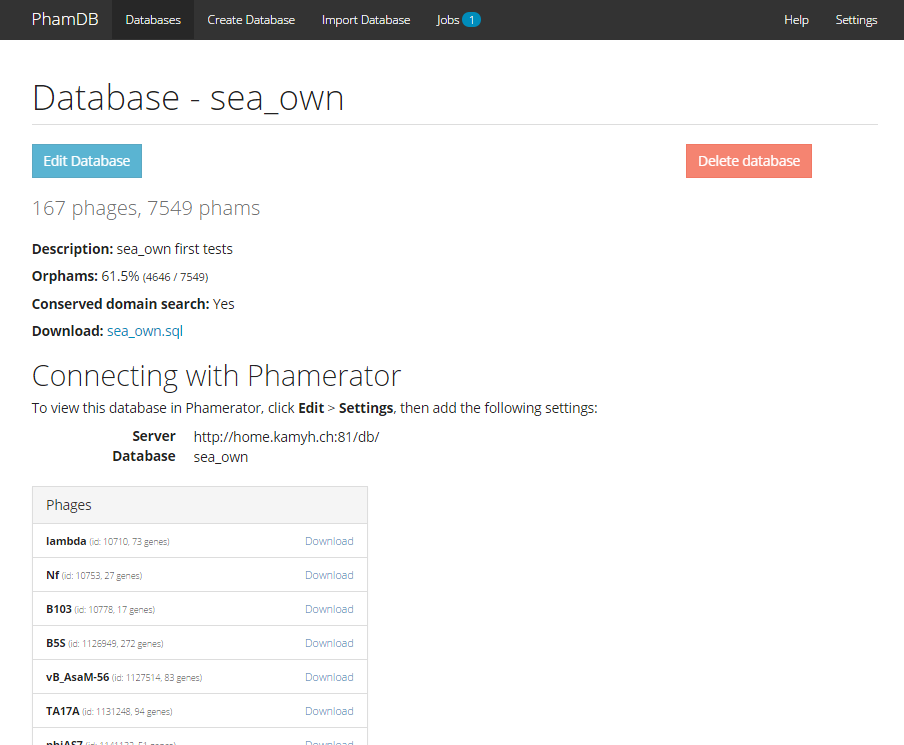
\includegraphics[scale=0.45]{img/phamdb_see_db}
		\caption{PhamDb database visualisation}
	\end{center}
\end{figure}

You can create a new database from three different ways:
\begin{enumerate}
	\item By importing phages from existing database on phamdb.
	\item By uploding Genbank files.
	\item By importing as an Sql file.
\end{enumerate}

\begin{figure}[H] 
	\begin{center}
		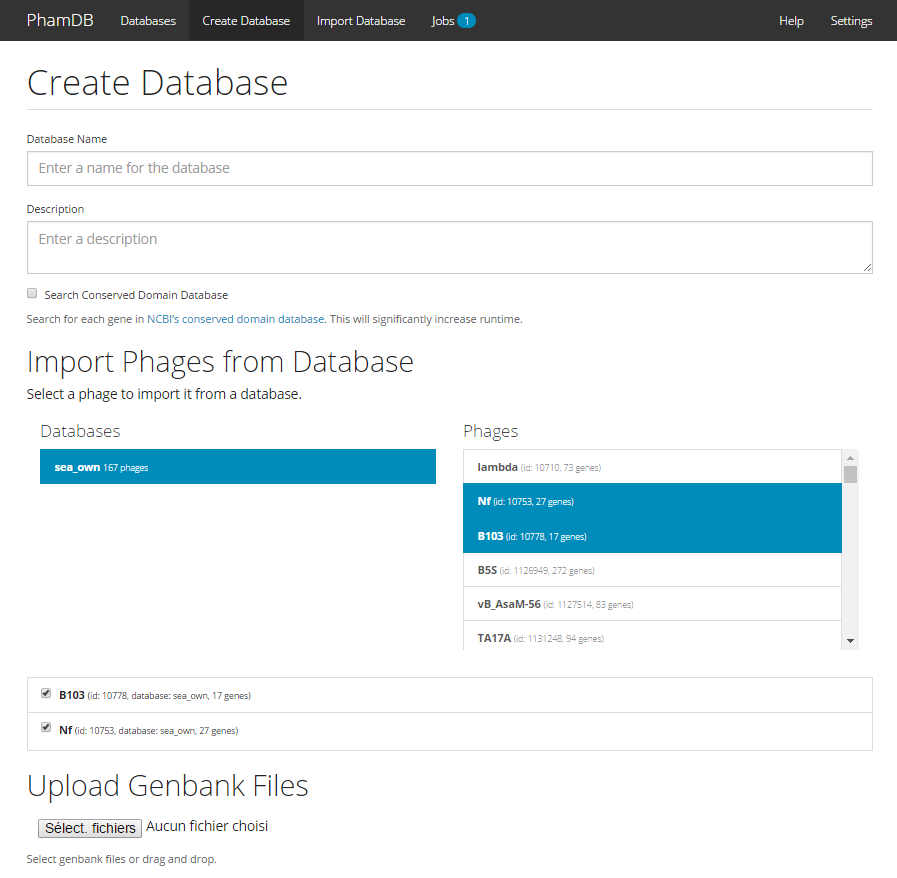
\includegraphics[scale=0.45]{img/phamdb_create_db}
		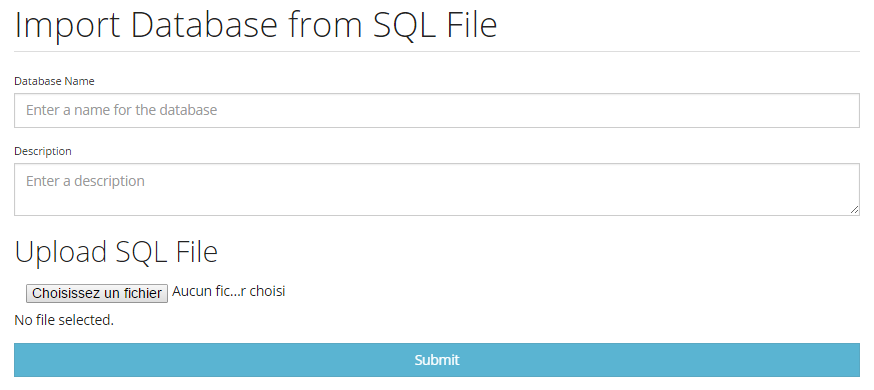
\includegraphics[scale=0.45]{img/phamdb_create_db_2}
		\caption{PhamDb database creation}
	\end{center}
\end{figure}

\section{Database \& Dataset}
We use the default database from phamerator for this phase of the project in order to gain some time. You can see the database structure on the figure 3.5 .

\begin{figure}[H] 
	\begin{center}
		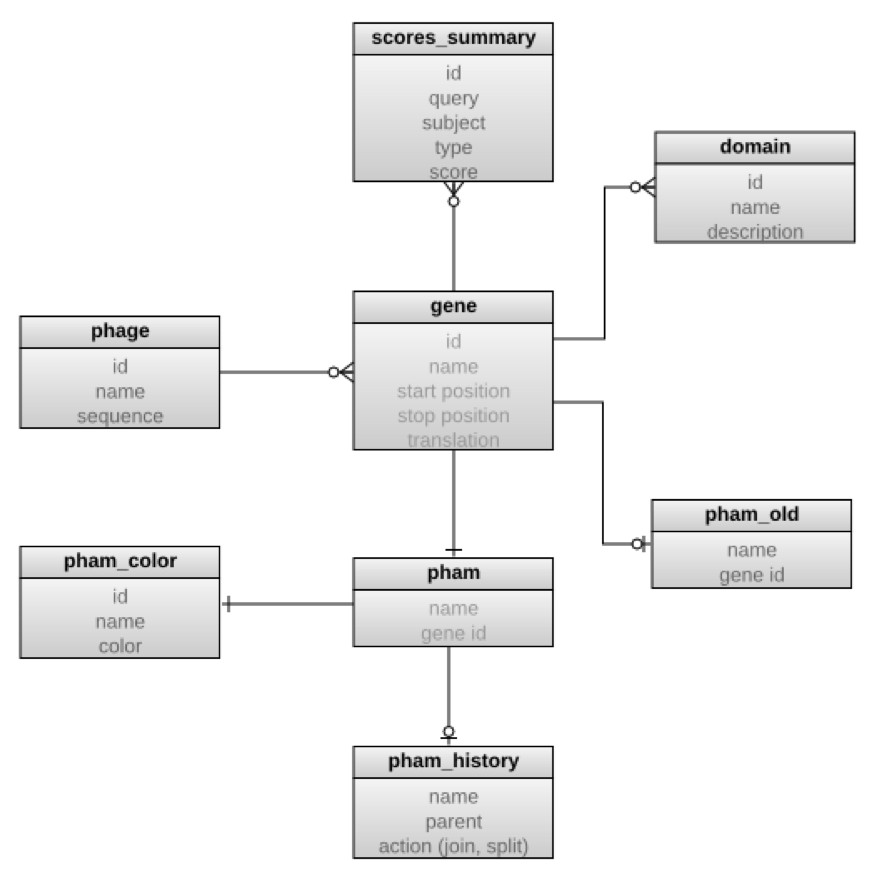
\includegraphics[scale=0.6]{img/12859_2011_Article_4954_Fig1_HTML}
		\caption{Docker harchitecture}
	\end{center}
\end{figure}

From the dataset at my disposal, I've used the list of phage "phages\_list\_1.txt". You can find it in annexe of this document.

\section{Phamily}
\subsection{Alignment}
\subsection{Phages selection}
\subsection{Data completion}


\chapter{Results \& Analyse}

\section{First result}
\subsection{Tree}
\subsection{Hosts}

\section{Database}
\subsection{SEA}
\subsection{Phages list integration}


\chapter{Conclusion}

\section{Problems encountered}
\subsection{Phamerator Installation}
\subsection{SEA database}
\subsection{PhamDB Limitation jobs}
\subsection{PhageDB.org}

\section{Perspectives}
\subsection{Database population}
\subsection{Resultats validation}
\subsection{Results by host}

\addtocounter{chapter}{1}
\addcontentsline{toc}{chapter}{\protect\numberline{\thechapter}References}
\bibliographystyle{plain} % Le style est mis entre accolades.
\bibliography{bibli} % mon fichier de base de données s'appelle bibli.bib


\chapter{Annexes}



\end{document}



